\pagestyle{fancy}
\headheight 20pt
\lhead{Ph.D. Thesis --- R. Woods }
\rhead{McMaster - Physics \& Astronomy}
\chead{}
\lfoot{}
\cfoot{\thepage}
\rfoot{}
\renewcommand{\headrulewidth}{0.1pt}
\renewcommand{\footrulewidth}{0.1pt}

\chapter{Applications to Galaxy Formation and Future Projects}
\label{chap:galaxyformation}
\thispagestyle{fancy}

We now use the algorithm described in chapter \ref{chap:method} and tested in chapter \ref{chap:codetests} to carry out simulations of an isolated galaxy. We have chosen to start with an isolated galaxy in order to probe the FUV field present in a [Milky Way-like... z=1?] disk in order to check if it is an important SF regulation mechanism.

FUV is an interesting band to start with for a few reasons. While FUV does not ionize gas, it is the primary driver of photoelectric heating \citep{tielens05}, which is the dominant heating mechanism for the ISM and the warm neutral medium. Despite this, very few astrophysical simulations actually include photoelectric heating due to its dependence on a radiation field.

As well, FUV is typically able to penetrate further into the ISM. At common densities in the ISM, an optical depth of 1 is typically only achieved after roughly one kpc. Current simulations, especially of isolated galaxies, can resolve distances much smaller than this, so looking at effects due to FUV is very feasible. On the other hand, bands such as EUV are usually absorbed within a few pc, a resolution that is very costly for even isolated galaxy simulations.

We have chosen to use an isolated galaxy IC from the AGORA galaxy comparison project \citep{kimEt14} to ensure use of a well-tested IC and provide a larger base for comparison of results.

\section{FUV Fields in the AGORA Disk}
\label{sec:agora}

The AGORA galaxy comparison project is a large computational comparison project that aims ``to raise the realism and predictive power of galaxy simulations and the understanding of the feedback processes that regulate galaxy `metabolism,' and by doing so to solve long-standing problems in galaxy formation'' \citep{kimEt14}. To accomplish this, the project has created both isolated and cosmological galaxy formation initial conditions at many different masses and resolutions, and has attempted to standardize physics modules and analysis methods for all of the codes involved in the project.

\subsection{Initial Conditions and Physics}
\label{sec:initialconditions}

We have chosen to run the isolated disk initial condition in order to examine FUV's effect on the ISM. The specific details of the ICs for this disk can be found in \citet{kimEt14}, section 2.2. We summarize here the important information.

The initial conditions have been generated at three different resolutions using the \textsc{MakeDisk} code, written by Volker Springel. The disk is created with four components: a dark matter halo, a gas disk, a stellar disk, and stellar bulge. The low resolution disk has $10^5$ DM particles, $10^5$ stellar disk particles, $10^5$ gas particles, and $1.24\e{4}$ stellar bulge particles. The medium and high resolution disks have 10 and 100 times more particles in each component, respectively.

The DM follows a NFW profile \citep{navarroEt97} with a concentration parameter $c = 10$ and a spin parameter $\lambda = 0.04$. The disk has an exponential profile with a scale length of $r_d = 3.432$ kpc and a scale height of $z_d = 0.1 r_d$. The disk is split into the stellar component, which has a mass of $4.297\e{10} M_{\odot}$, and a gas component, which has a mass of 20\% of the DM mass. The stellar bulge follows the Hernquist \citeyear{hernquist90} density profile with a bulge-to-disk mass ratio of B/D = 0.1. Gas is initiated at $10^4$ K. The \textsc{MakeDisk} code ensures that the above conditions give quasi-equilibrium [what does that mean?] for the four components. 

We have run the IC for 335~Myr in order to make sure it was relaxed, and started all subsequent runs from this point. An image of the relaxed IC is shown in figure \ref{fig:agoraic}.

\begin{figure}
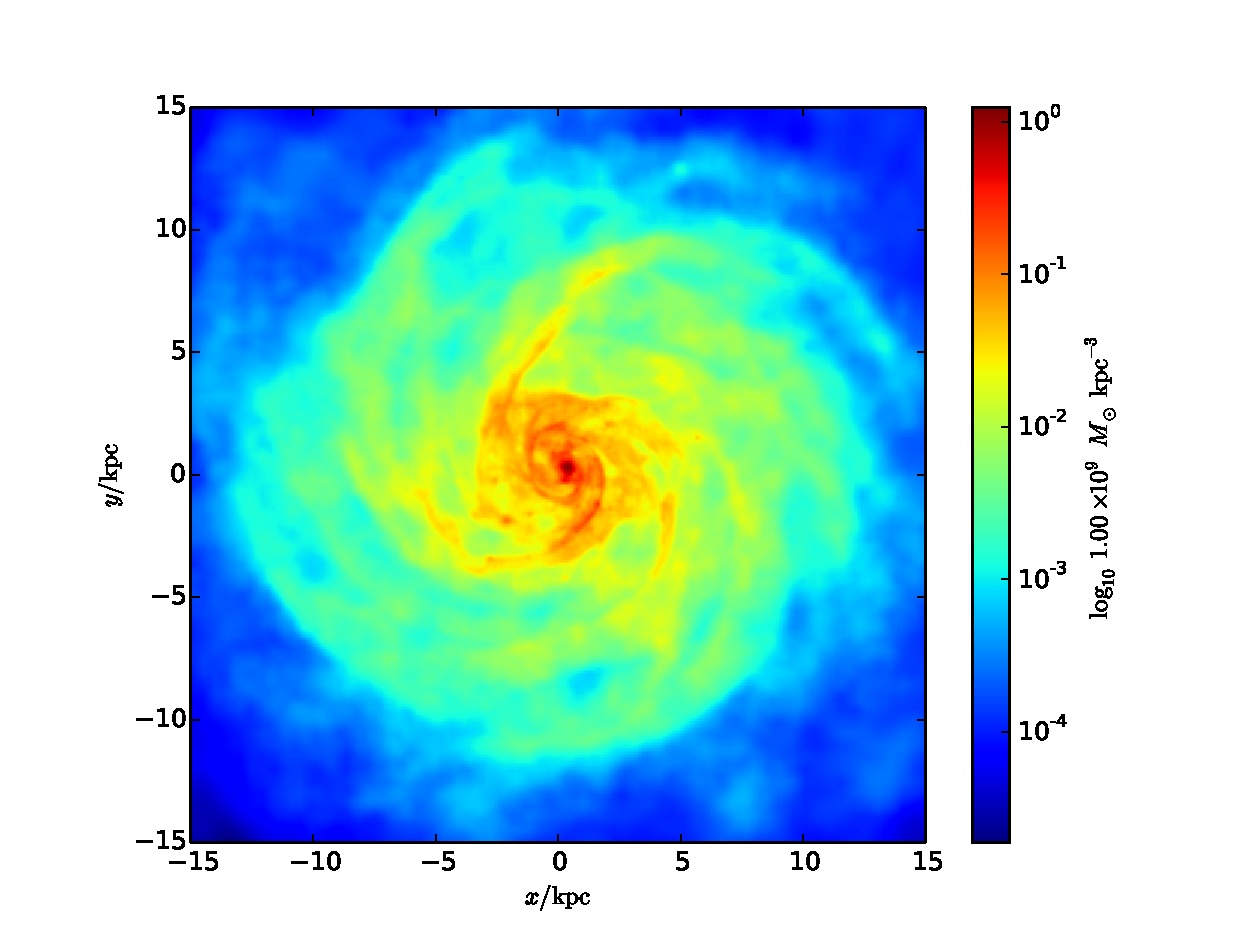
\includegraphics[width=\textwidth]{graphics/AGORAic.eps}
\caption[The AGORA IC]{A density projection of a relaxed version of the AGORA initial condition. We have run the IC for 335 Myr in order to relax it.}
\label{fig:agoraic}
\end{figure}

%notes about various runs we did

We have run the low resolution simulation with a number of different physical parameters, including our radiative transfer with FUV, a background FUV at two intensities (the standard for most codes without radiative transfer), Supernovae (SNe) feedback \citep{kellerEt14}, and a number of different opacities. Table \ref{tab:simsummary} summarizes the simulations and the names we have given them.

\begin{table}
\begin{tabular}{lllll}
Name & RT & UV Strength (units?) & Opacity (g/cm$^{-2}$) & SNe Feedback\\ \hline \hline
FUV0 & No & 0 & 0 & No\\
FUV & Yes & 0 & 300 & No\\
FUVop100 & Yes & 0 & 100 & No\\
FUVthin & Yes & 0 & 0 & No\\
FUV2e-26 & No & 2e-26 & 300 & No\\u? This is amazing and looks extremely difficult to recreate
permalink
[–]BlindStark 20 points 2 hours ago 
There is an achievement hunter video where they jump from helicopters to do
FUV2e-27 & No & 2e-27 & 300 & No\\
FB & No & ? & 300 & yes\\
FB\_FUV & Yes & 0 & 300 & yes\\
FB\_FUV2e-26 & No & 2e-26 & 300 & yes\\
FB\_FUV2-27 & No & 2e-27 & 300 & yes\\
\hline
\end{tabular}
\caption[Summary of simulations]{A summary of the simulations that were run.}
\label{tab:simsummary}
\end{table}

We attempted to match opacities given in \citet{wolfireEt03}. The left pane of figure \ref{fig:wolfiresummary} shows the midplane HI density and absorption coefficient, and the right pane is the inferred opacity from the left pane, obtained by dividing absorption by mass density.

\begin{figure}
        \centering
        \begin{subfigure}[b]{0.45\textwidth}
                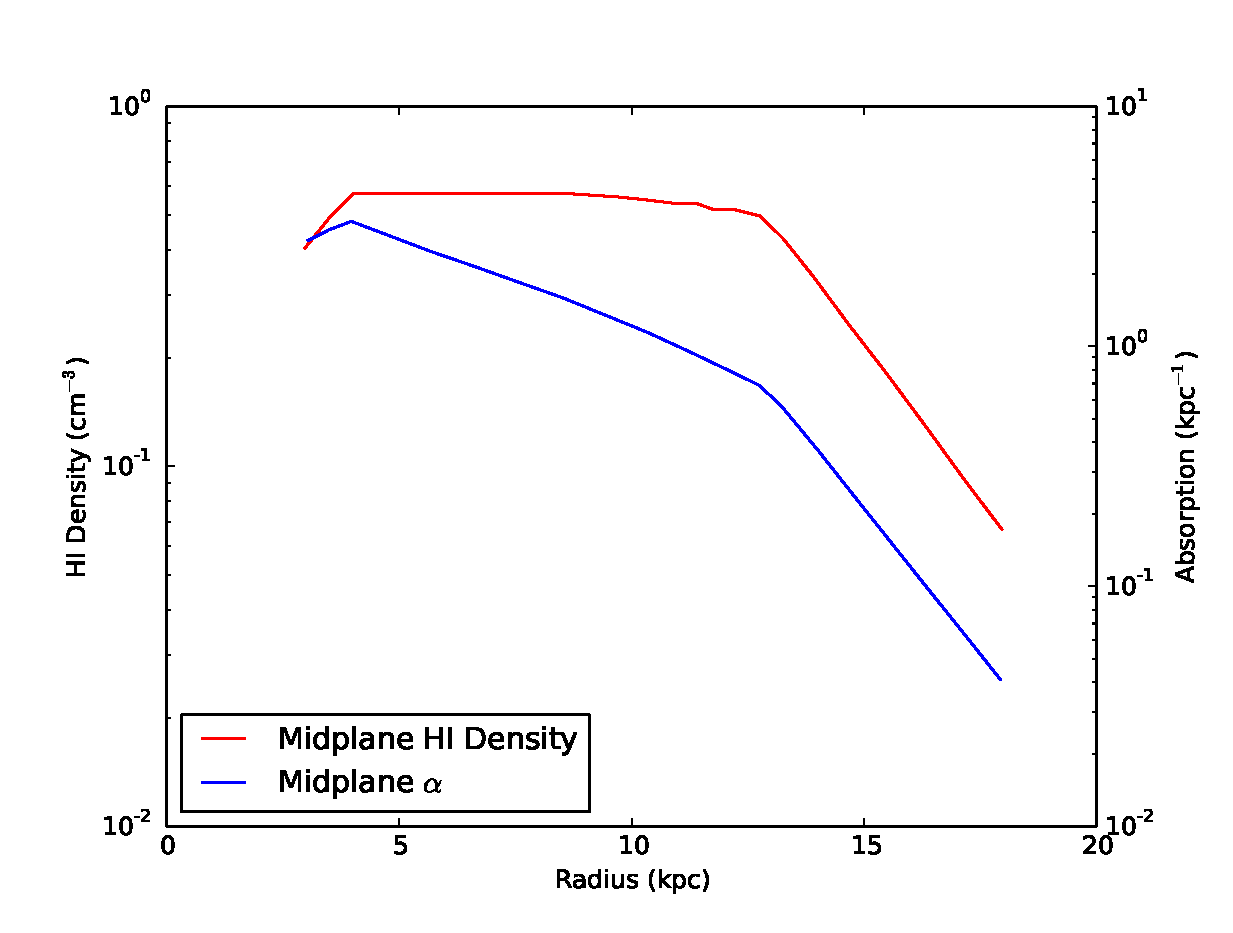
\includegraphics[width=\textwidth]{graphics/densityabsorptionvr.eps}
        \end{subfigure}
        ~ 
        \begin{subfigure}[b]{0.45\textwidth}
                \includegraphics[width=\textwidth]{graphics/opacityvr.eps}
        \end{subfigure}
        \caption[Parameters from \citet{wolfireEt03}.]{Parameters from \citet{wolfireEt03}. The left plot shows the mid plane number density and absorption coefficient. The right plot is obtained by converting number density to a mass density and dividing absorption coefficient by mass density.}
        \label{fig:wolfiresummary}
\end{figure}

Note that the profile in opacity is due solely to a scaling in metallicity of the local opacity. \citet{wolfireEt03} assume that opacity changes as

\begin{equation}
\kappa = \kappa_{\odot}\left(\frac{Z}{Z_{\odot}}\right),
\end{equation}

where $\kappa_{\odot}$ is the metallicity in the solar neighborhood, inferred to be ~400 g/cm$^{-2}$ from figure \ref{fig:wolfiresummary}.

We have also included a run at eight times higher resolution to check on convergence of results. These runs are prefixed with an ``8''.

\section{The Role of FUV on Star Formation}
\label{sec:fuvsfr}



%\begin{figure}
%        \centering
%        \begin{subfigure}[b]{0.3\textwidth}
%                \includegraphics[width=\textwidth]{graphics/surfacedensityRadFUV0_J300080.eps}
%                \caption{FUV0}
%                \label{fig:intensitythin}
%        \end{subfigure}
%        ~
%        \begin{subfigure}[b]{0.3\textwidth}
%                \includegraphics[width=\textwidth]{graphics/surfacedensityRadFUV2e-26_J300080.eps}
%                \caption{FUV2e-26}
%                \label{fig:intensity100}
%        \end{subfigure} 
%        ~ 
%        \begin{subfigure}[b]{0.3\textwidth}
%                \includegraphics[width=\textwidth]{graphics/surfacedensityRadFUVop400_J300080.eps}
%                \caption{FUVop400}
%                \label{fig:intensity100}
%        \end{subfigure}
%        \\
%        \begin{subfigure}[b]{0.3\textwidth}
%                \includegraphics[width=\textwidth]{graphics/surfacedensityRadFUV_J300080.eps}
%                \caption{FUVop300}
%                \label{fig:intensitythin}
%        \end{subfigure}
%        ~
%        \begin{subfigure}[b]{0.3\textwidth}
%                \includegraphics[width=\textwidth]{graphics/surfacedensityRadFUVop100_J300080.eps}
%                \caption{FUVop100}
%                \label{fig:intensitythin}
%        \end{subfigure}
%        ~
%        \begin{subfigure}[b]{0.3\textwidth}
%                \includegraphics[width=\textwidth]{graphics/surfacedensityRadFUVthin_J300080.eps}
%                \caption{FUVthin}
%                \label{fig:intensitythin}
%        \end{subfigure}
%        \\
%         \begin{subfigure}[b]{0.3\textwidth}
%                \includegraphics[width=\textwidth]{graphics/surfacedensityRadFB_J300080.eps}
%                \caption{FB}
%                \label{fig:intensity100}
%        \end{subfigure}
%        ~ 
%        \begin{subfigure}[b]{0.3\textwidth}
%                \includegraphics[width=\textwidth]{graphics/surfacedensityRadFB_FUV2e-26_J300080.eps}
%                \caption{FB\_FUV2e-26}
%                \label{fig:intensitythin}
%        \end{subfigure}
%        ~
%        \begin{subfigure}[b]{0.3\textwidth}
%                \includegraphics[width=\textwidth]{graphics/surfacedensityRadFB_FUV_J300080.eps}
%                \caption{FB\_FUV}
%                \label{fig:intensitythin}
%        \end{subfigure}
%        \caption[Surface density for varying runs.]{Surface density plots for the different runs.}
%        \label{fig:intensityvopacity}
%\end{figure}

%\begin{figure}
%        \centering
%        \begin{subfigure}[b]{0.45\textwidth}
%                \includegraphics[width=\textwidth]{graphics/fluximageRadFUV_J300080.eps}
%                \caption{FUVop300}
%                \label{fig:intensitythin}
%        \end{subfigure}
%        ~
%        \begin{subfigure}[b]{0.45\textwidth}
%                \includegraphics[width=\textwidth]{graphics/fluximageRadFUVthin_J300080.eps}
%                \caption{FUVthin}
%                \label{fig:intensity100}
%        \end{subfigure}        
%        \\
%        \begin{subfigure}[b]{0.45\textwidth}
%                \includegraphics[width=\textwidth]{graphics/fluximage8_RadFUV_J300080.eps}
%                \caption{8\_FUVop300}
%                \label{fig:intensitythin}
%        \end{subfigure}
%        ~
%        \begin{subfigure}[b]{0.45\textwidth}
%                \includegraphics[width=\textwidth]{graphics/fluximage8_RadFUVthin_J300080.eps}
%                \caption{8\_FUVthin}
%                \label{fig:intensitythin}
%        \end{subfigure}        
%        \\ 
%        \begin{subfigure}[b]{0.45\textwidth}
%                \includegraphics[width=\textwidth]{graphics/fluximageRadFUVop400_J300080.eps}
%                \caption{FUVop400}
%                \label{fig:intensity100}
%        \end{subfigure}
%        ~
%        \begin{subfigure}[b]{0.45\textwidth}
%                \includegraphics[width=\textwidth]{graphics/fluximageRadFB_FUV_J300080.eps}
%                \caption{FB\_FUVop300}
%                \label{fig:intensitythin}
%        \end{subfigure}    
%        \caption[Mass-weighted intensity.]{Mass-weighted intensity of the different runs.}
%        \label{fig:intensityvopacity}
%\end{figure}

We begin by looking at the star formation history of each simulation. Figure \ref{fig:sfrvtime} shows the star formation rate as a function of time for each simulation. 

%\begin{figure}
%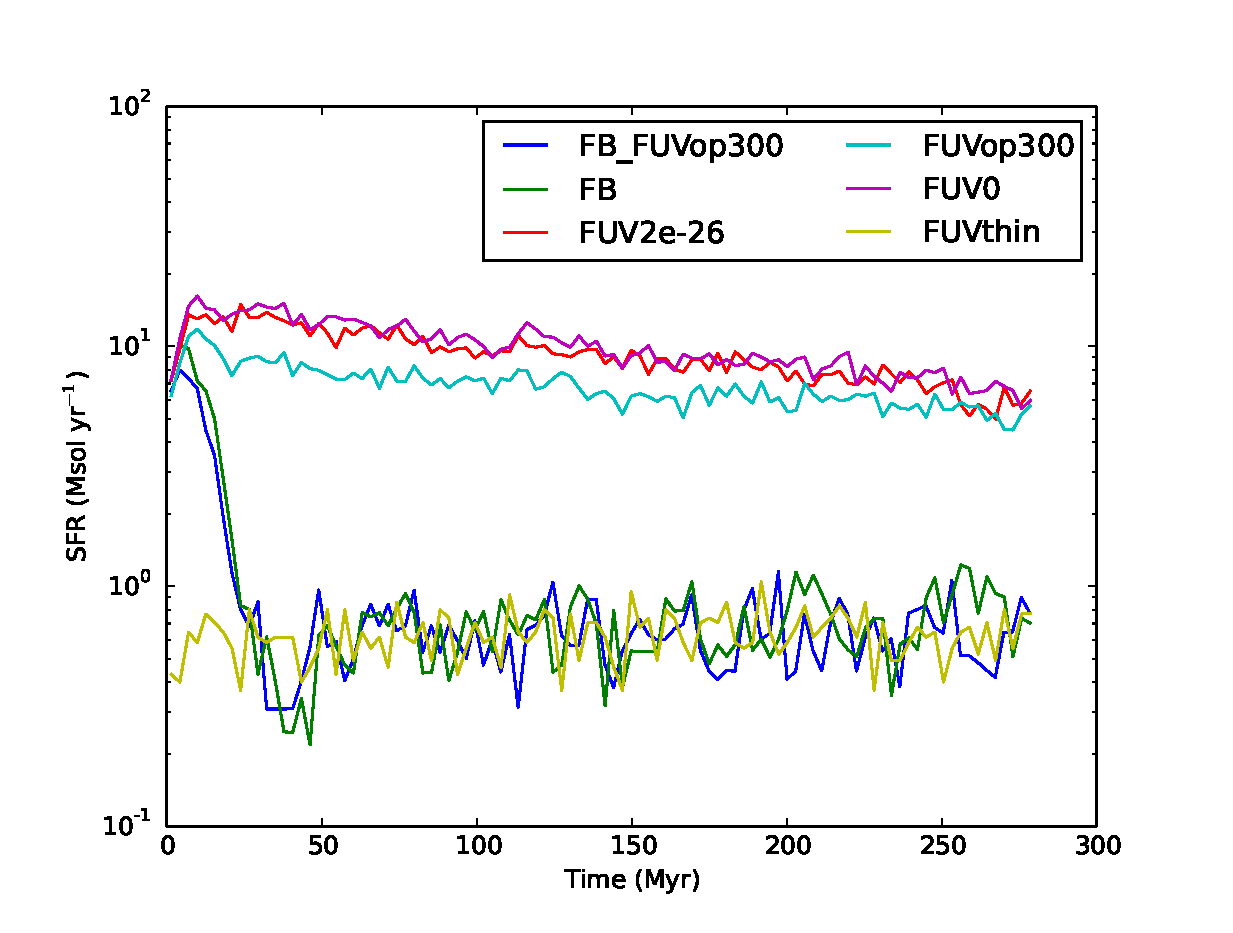
\includegraphics[width=\textwidth]{graphics/sfrvtime.eps}
%\caption[Star formation histories.]{Star formation rate vs time for each simulation. Feedback dominates the star formation regulation in this galaxy. Looking only at FUV, local feedback has a noticeable effect over a uniform background UV field.}
%\label{fig:sfrvtime}
%\end{figure}

It is clear that SNe feedback has a very strong regulation effect on star formation, as the rate in all runs with SNe feedback is about a factor of five lower than simulations without SNe feedback. In runs without SNe feedback, local FUV fields tend to reduce star formation rates by a factor of around 25\% compared to uniform backgrounds. Comparing the RadFUV2e-26 and RadFUV2e-27, there is no noticeable difference, suggesting that the FUV due to a uniform background has no ability to regulate star formation.

We must check whether the FUV field present in the galaxy is similar to observations. Figure \ref{fig:intensitywolfire} is a plot of FUV intensity vs radius in the midplane of the galaxy.

%\begin{figure}
%\includegraphics[width=\textwidth]{graphics/intensityvrRadFUV_J300080.eps}
%\caption[FUV intensity vs radius]{FUV intensity vs radius in the galaxy midplane for the RadFUV case. The dots are individual particle fluxes and the solid line is from figure 5.5 of \citet{wolfireEt03}.}
%\label{fig:intensitywolfire}
%\end{figure}

The points are intensities for individual particles and the lines is the mean intensity presented in \citet{wolfireEt03}. On average, the FUV intensity seen by a particle is far lower than the mean field presented by \citet{wolfireEt03}. We can examine the runs with varying opacity to see how this effects to local FUV intensity as well as the SFR.

%\begin{figure}
%        \centering
%        \begin{subfigure}[b]{0.45\textwidth}
%                \includegraphics[width=\textwidth]{graphics/intensityvrRadFUVop100_J300080.eps}
%                \caption{FUVop100}
%                \label{fig:intensity100}
%        \end{subfigure}
%        ~ 
%        \begin{subfigure}[b]{0.45\textwidth}
%                \includegraphics[width=\textwidth]{graphics/intensityvrRadFUVthin_J300080.eps}
%                \caption{FUVthin}
%                \label{fig:intensitythin}
%        \end{subfigure}
%        \caption[Intensity with varying opacity.]{FUV intensity vs radius in the galaxy midplane for $\kappa = 100$ g/cm$^{-2}$ and for an optically thin medium.}
%        \label{fig:intensityvopacity}
%\end{figure}

We see that opacity, not surprisingly, makes a large difference in the mean intensity seen by particles. However, what's notable is that even in the optically thin case, we are unable to attain the intensity levels reported in \citet{wolfireEt03}.

It is worth revisiting the star formation histories of the new simulations. Figure \ref{fig:sfrvtimeRT} shows the star formation histories for various runs with RT.

%\begin{figure}
%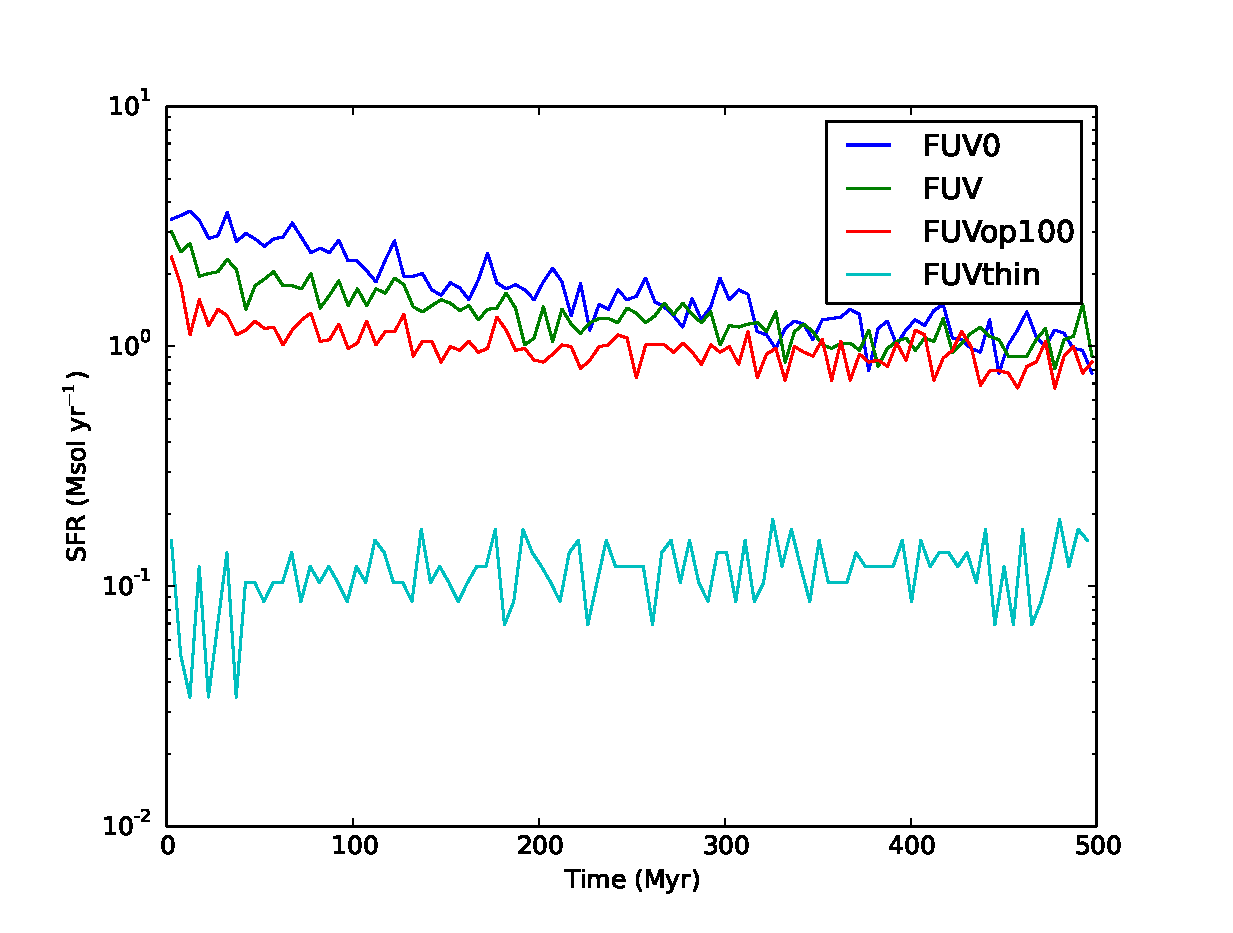
\includegraphics[width=\textwidth]{graphics/sfrvtimeRT.eps}
%\caption[Star formation histories for varying opacities.]{Star formation rate vs time with varying opacity. While the assumed opacity value of 400 g/cm,$^{-2}$ gives very minimal regulation in star formation, an optically thin approximation gives incredibly strong regulation. An opacity of 100 $g/cm^{-2}$ gives the most reasonable star formation rate, if comparing to the Milky Way.}
%\label{fig:sfrvtimeRT}
%\end{figure}

In the optically thin case, we see how important FUV can be at regulating star formation when intensities are much higher. Even lowering opacity to 100 g/cm$^{-2}$ makes a very significant difference, and gives a star formation rate in agreement with the Milky Way.

In order to understand the affect FUV has on gas, we consider phase diagrams for gas in the galaxy. Figure \ref{fig:phasediagrams} shows phase diagrams of gas in a number of the different simulations.

%\begin{figure}
%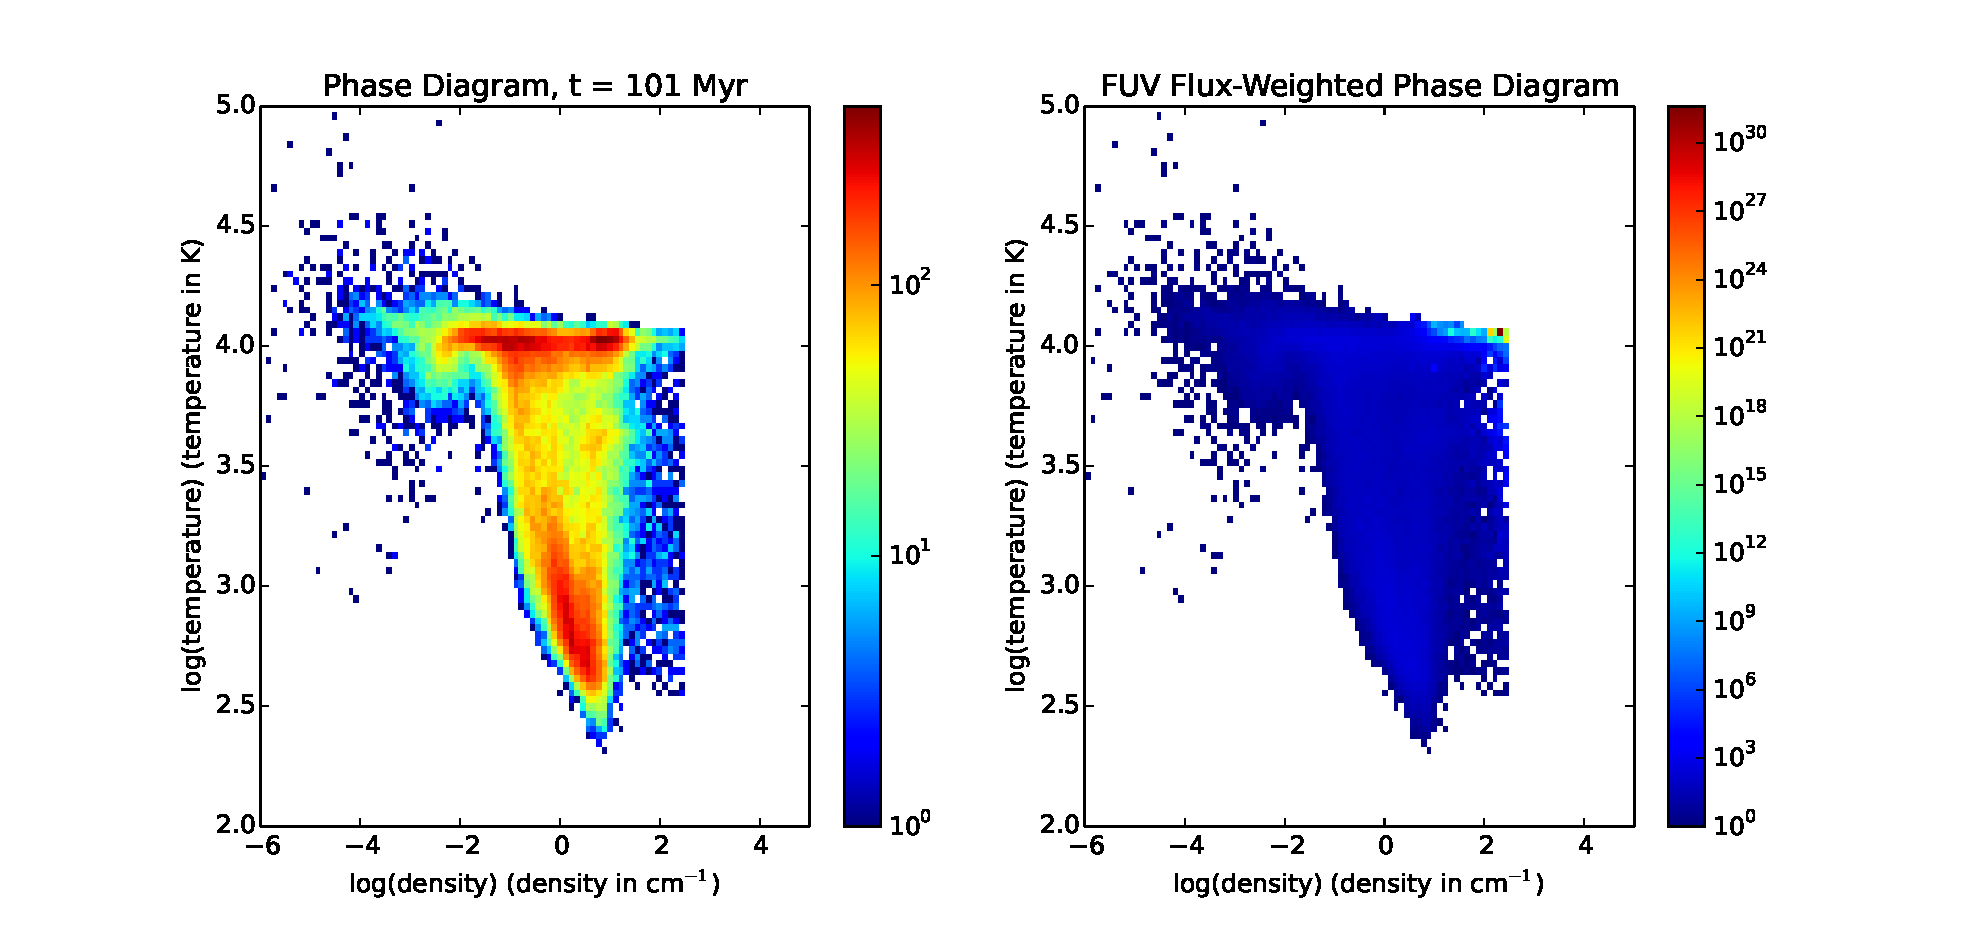
\includegraphics[width=\textwidth]{graphics/phaseRadFUV00101.eps}
%\caption[Phase diagrams with different physics]{Phase diagrams for each simulation case.}
%\label{fig:phasediagrams}
%\end{figure}

In cases with FUV simulated with radiative transfer, a portion of the gas is seen to be heated to about $10^4$ K around densities of 100 atoms cm$^{-3}$.

[Add commentary. Re-radiation important? Clumpy medium vs average opacity not the same.]